\subsection{Обоснование архитектурного шаблона проектирования}
\label{sub:system-design:architectural-pattern-design}

На сетевом уровне, предполагающем рассмотрение взаимодействия различных систем через сеть, в основе разрабатываемой системы лежит архитектура «клиент-сервер», в которой задания или сетевая нагрузка распределены между поставщиками услуг (сервисов), называемых серверами, и заказчиками услуг, называемых клиентами. В качестве среды взаимодействия клиента с сервером используется сеть Интернет. На рис.~\ref{fig:client-server-architecture} показана диаграмма, отражающая взаимосвязь компонентов клиент-серверной архитектуры.

\begin{figure}[h]
\centering
    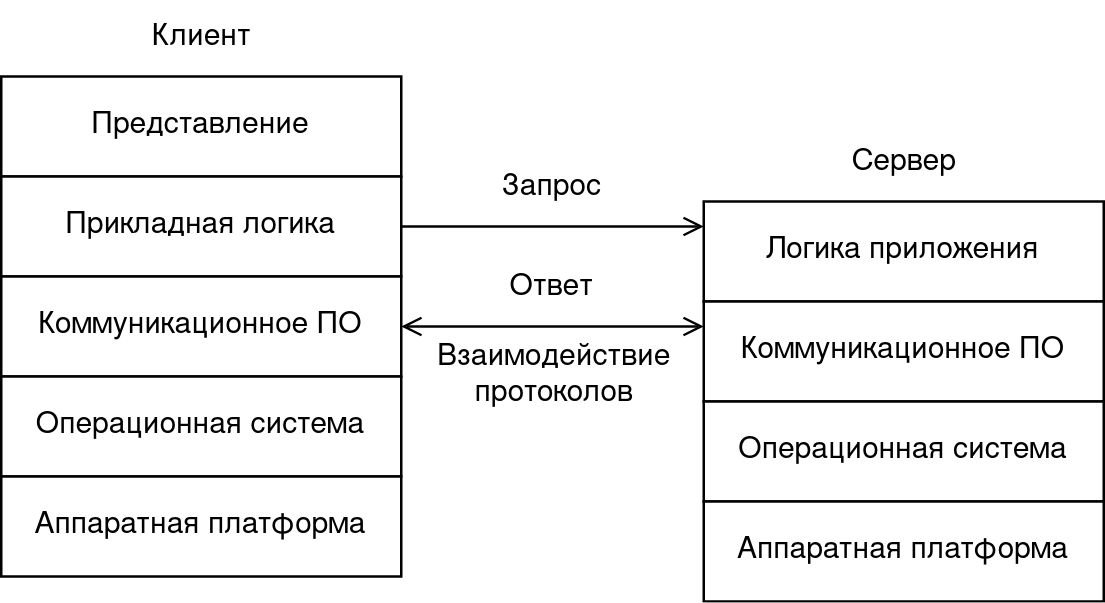
\includegraphics[width=0.75\linewidth]{assets/client-server-architecture.png}
    \caption{Схема архитектуры «клиент-сервер»}
    \label{fig:client-server-architecture}
\end{figure}

Основными достоинствами архитектуры «клиент-сервер» являются:

\begin{itemize}
    \item возможность, в большинстве случаев, распределить функции вычислительной системы между несколькими независимыми компьютерами в сети, что позволяет упростить обслуживание вычислительной системы, в частности, замена, ремонт, модернизация или перемещение сервера, не затрагивают клиентов;
    \item обеспечение хранения данных только на сервере, который, как правило, защищён гораздо лучше большинства клиентов, что позволит обеспечить контроль полномочий, чтобы разрешать доступ к данным только клиентам с соответствующими правами доступа;
    \item возможность объединения клиентов с разными аппаратными платформами, операционными системами для использования ресурсов одного сервера.
\end{itemize}

К основным недостаткам клиент-серверной архитектуры можно отнести:

\begin{itemize}
    \item неработоспособность основного сервера, в случае использования централизованной системы, может сделать неработоспособным всё приложение;
    \item потребность в наличии квалифицированного профессионала для администрирования системы;
    \item высокая стоимость оборудования.
\end{itemize}

В ходе выбора аппаратной платформы в данном дипломном проекте будут предложены и реализованы решения, позволяющие минимизировать вероятность выхода из строя серверной части приложения, а также позволяющие снизить стоимость оборудования до оплаты минимально необходимого уровня производительности.

Реализация серверной части системы, содержащей бизнес-логику и программный код, выполнена в соответствии с микросервисной архитектурой, которая представляет собой стиль разработки программного обеспечения, при котором система строится как набор небольших, автономных сервисов, каждый из которых отвечает за конкретный функциональный блок или бизнес-операцию. Единицей модульности является сервис. Сервис~-- это автономный, независимо развертываемый программный компонент, который реализует определенные полезные функции~\cite{book_microservices_patterns}. Схема микросервисной архитектуры представлена на рис.~\ref{fig:system-design:architectural-pattern-design:microservice-architecture}. В качестве коннекторов служат коммуникационные протоколы, которые позволяют сервисам взаимодействовать между собой.

\begin{figure}[h]
\centering
    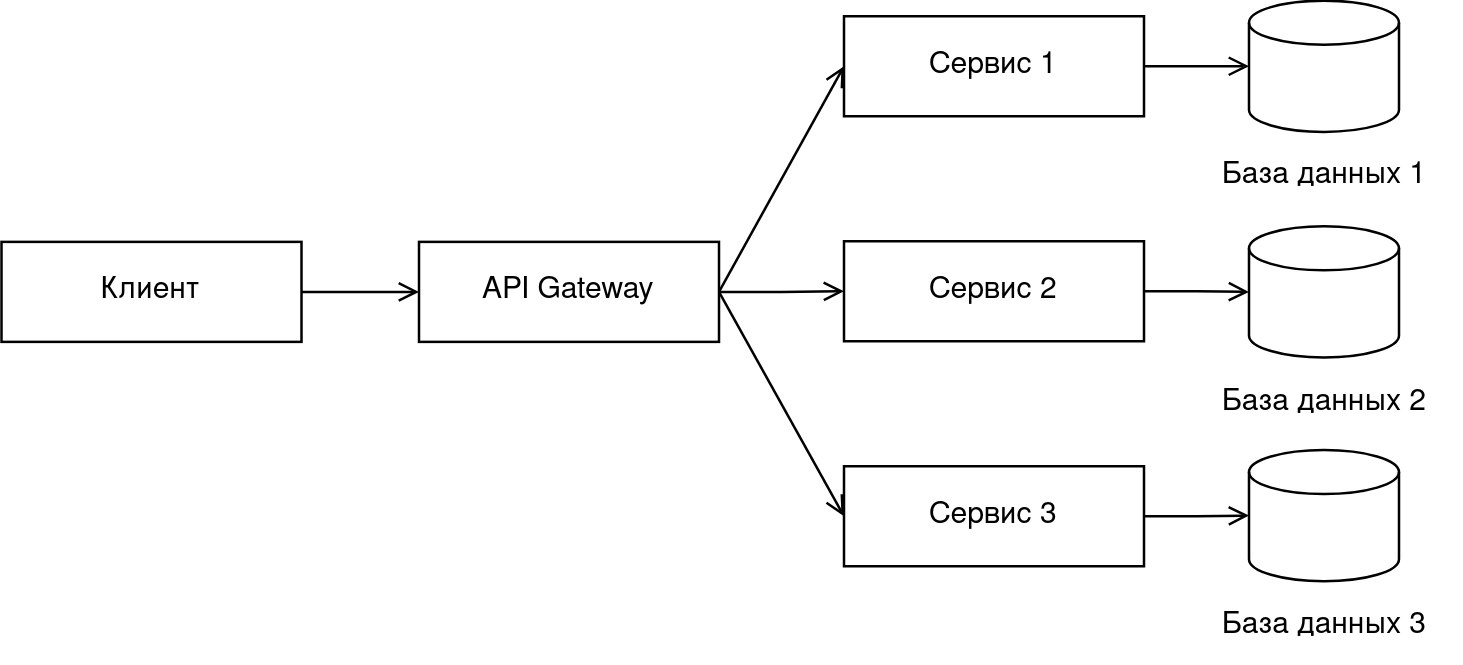
\includegraphics[width=0.9\linewidth]{assets/microservice-architecture.png}
    \caption{Схема микросервисной архитектуры}
    \label{fig:system-design:architectural-pattern-design:microservice-architecture}
\end{figure}

Основной стратегией создания микросервисной архитектуры является разбиение по бизнес-возможностям (поддоменам в предметно-ориен\-ти\-ро\-ван\-ном программировании). На рис.~\ref{fig:microservices-service-illustration} показано внешнее представление сервиса (в данном случае \textit{OfficeManagement}). Сервис обладает \textit{API}, который инкапсулирует реализацию. \textit{API} определяет операции, вызываемые клиентами. Существует два типа операций: команды (обновляют данные) и запросы (извлекают данные). При изменении своих данных сервис публикует события, на которые могут подписаться его клиенты. \textit{API} состоит из команд, запросов и событий. Команда, такая как \textit{\lstinline!create_workspace()!}, выполняет действия и обновляет данные. Запрос, такой как \textit{\lstinline!find_workspace()!}, извлекает данные. Сервис также публикует события, например
\textit{\lstinline!WorkspaceCreated!}, которые потребляются его клиентами. \textit{API} сервиса, который реализуется адаптерами, которые взаимодействуют с бизнес-логикой приложения, инкапсулирует его внутреннюю реализацию.

\begin{figure}[h]
\centering
    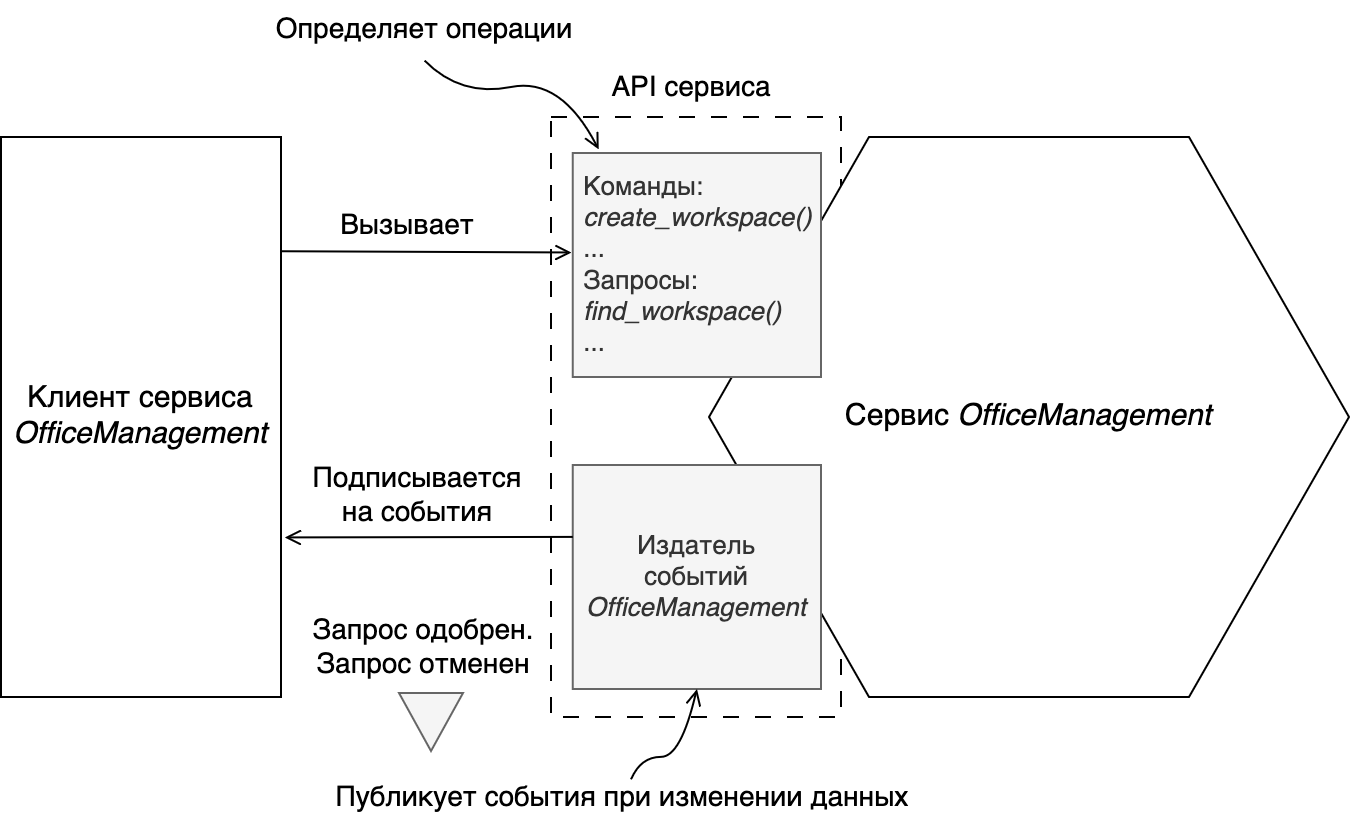
\includegraphics[width=0.9\linewidth]{assets/microservices-service-illustration.png}
    \caption{Внешнее представление сервиса \textit{OfficeManagement}}
    \label{fig:microservices-service-illustration}
\end{figure}

Достоинствами микросервисной архитектуры являются:

\begin{itemize}
    \item наличие возможности непрерывной доставки и независимого развертывания крупных, сложных приложений;
    \item сервисы получаются небольшими и простыми в обслуживании;
    \item позволяет экспериментировать и внедрять новые технологии;
    \item в ней лучше изолированы неполадки.
\end{itemize}

Возможность выполнять непрерывные доставку и развертывание обеспечивает несколько бизнес-преимуществ, например: компания обеспечивает уровень надежности своих услуг, соответствующий современным ожиданиям; работники довольны, поскольку вместо реализации сложных интеграций новых возможностей с существующей логикой они уделяют больше времени выпуску нового функционала.

Определение обязанностей каждого программного элемента является одной из основных задач проектирования программных продуктов. Принцип единственной ответственности \textit{SRP} гласит о том, что у класса должна быть только одна причина для изменения. Применяя \textit{SRP} к микросервисной архитектуре, получим совокупность небольших согласованных сервисов, обладающих одной обязанностью. Принцип согласованного изменения \textit{CCP} гласит о том, что причины изменения классов, входящих в один пакет, должны быть одинаковыми. Изменение пакета должно затрагивать все его классы. \textit{CCP} можно применить при создании микросервисной архитектуры, объединяя компоненты, изменяющиеся по одной и той же причине, в единый сервис, что позволит сократить количество сервисов, которые придется редактировать и заново развертывать при изменении какого-либо бизнес-требования.

Все сервисы и их \textit{API} имеют четкие определения. Каждый из них можно разрабатывать, тестировать, развертывать и масштабировать независимо от остальных. Такая архитектура помогает поддерживать модульность. Разработчик не может обратиться к внутренним компонентам сервиса, минуя его \textit{API}.

Важным шагом в определении архитектуры приложения является описание \textit{API} для каждого сервиса. Это реализуется путем назначения сервисам всех системных операций, определенных в перечне функциональных требований. Операция может быть реализована в виде одного или нескольких сервисов. В последнем случае необходимо решить, как они будут взаимодействовать между собой, что обычно требует поддержки дополнительных операций с их стороны. Также необходимо выбрать один из механизмов \textit{IPC}, чтобы реализовать \textit{API} каждого из сервисов.

После описания обобщенной доменной модели необходимо определить перечень запросов, которые приложение должно обрабатывать. В реализуемой системе большинство запросов основаны на \textit{HTTP}, однако вполне вероятно, что некоторым клиентам необходим механизм обмена сообщениями. Таким образом, вместо привязки к конкретному протоколу для представления запросов лучше использовать более абстрактное понятие системной операции~\cite{book_microservices_patterns}.

Системные операции бывают двух типов:
\begin{itemize}
    \item \textit{команды}~-- системные операции для создания, обновления и удаления данных;
    \item \textit{запросы}~-- системные операции для чтения (запрашивания) данных.
\end{itemize}

Бизнес-логика реализуемой системы состоит из нескольких бэкенд-сервисов. У каждого из них есть \textit{REST API} и собственная приватная база данных. Схема соответствия между бизнес-возможностями и сервисами разрабатываемой системы показана на рис.~\ref{fig:system-design:architectural-pattern-design:microservices-business-use-case}. Сервисам соответствуют возможности разных уровней иерархии.

\begin{figure}
\centering
    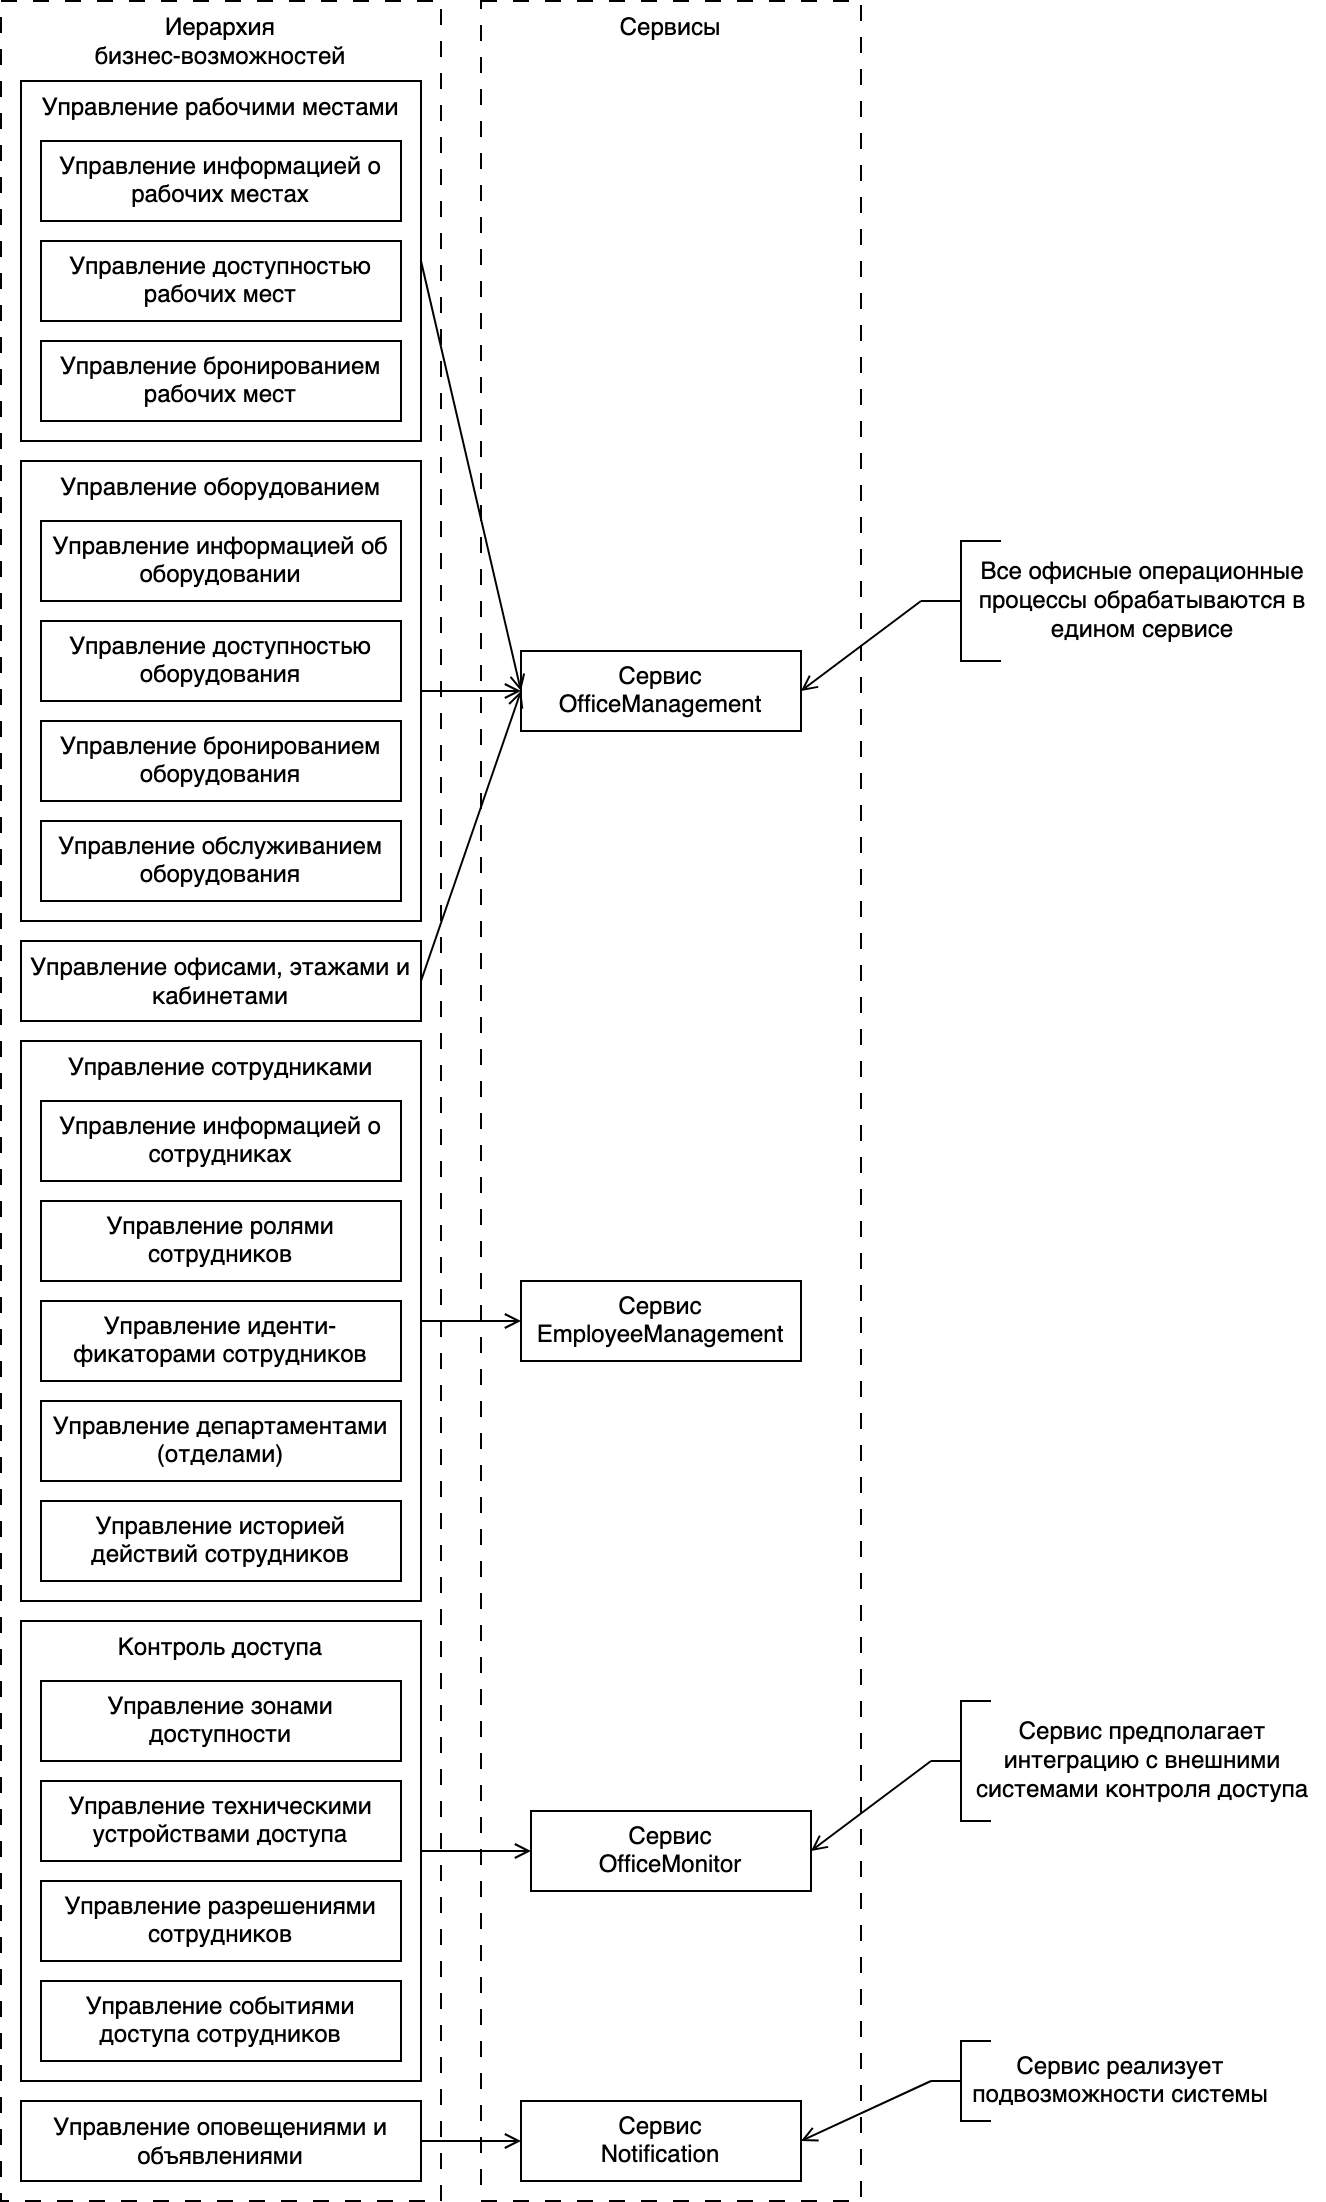
\includegraphics[width=0.8\linewidth]{assets/microservices-business-use-cases.png}
    \caption{Схема соответствия бизнес-возможностей и сервисов разрабатываемой системы}
    \label{fig:system-design:architectural-pattern-design:microservices-business-use-case}
\end{figure}

Сервисами системы являются:

\label{page:system-design:architectural-pattern-design:microservices-list}
\begin{itemize}
    \item \textit{EmployeeManagement} - управляет сотрудниками;
    \item \textit{OfficeManagement} - управляет операционными процессами;
    \item \textit{OfficeMonitor} - управляет контролем доступа и посещаемости;
    \item \textit{Notification} - отвечает за отправку уведомлений пользователям системы.
\end{itemize}

Иногда сервисы создаются для возможностей верхнего уровня, таких как управление рабочими местами или контроль доступа, а иногда~-- для подвозможностей, например, управление оповещениями и объявлениями.

Сервисы могут взаимодействовать через \textit{API}: примитивные каналы, такие как брокеры сообщений или простые протоколы, подобные \textit{REST} или \textit{gRPC}. Асинхронный \textit{API} состоит из операций, вызываемых клиентами, и событий, которые публикуют сервисы. В реализуемой системе используется подход с использованием асинхронного обмена сообщениями, что имеет неоспоримое преимущество~-- отсутствие блокировки клиента в ожидании ответа с расчетом на то, что ответ может прийти не сразу. Как видно на рис.~\ref{fig:microservices-broker-messaging}, сообщения передаются по каналам. Бизнес-логика отправителя обращается к интерфейсу исходящего порта, который реализуется адаптером отправителя сообщения. Отправитель шлет сообщение получателю через канал. Канал сообщений~-- это абстракция инфраструктуры обмена сообщениями. Адаптер обработчика сообщений в получателе вызывается для обработки сообщения. Он обращается к интерфейсу входящего порта, который реализуется бизнес-логикой получателя.

\begin{figure}[h]
\centering
    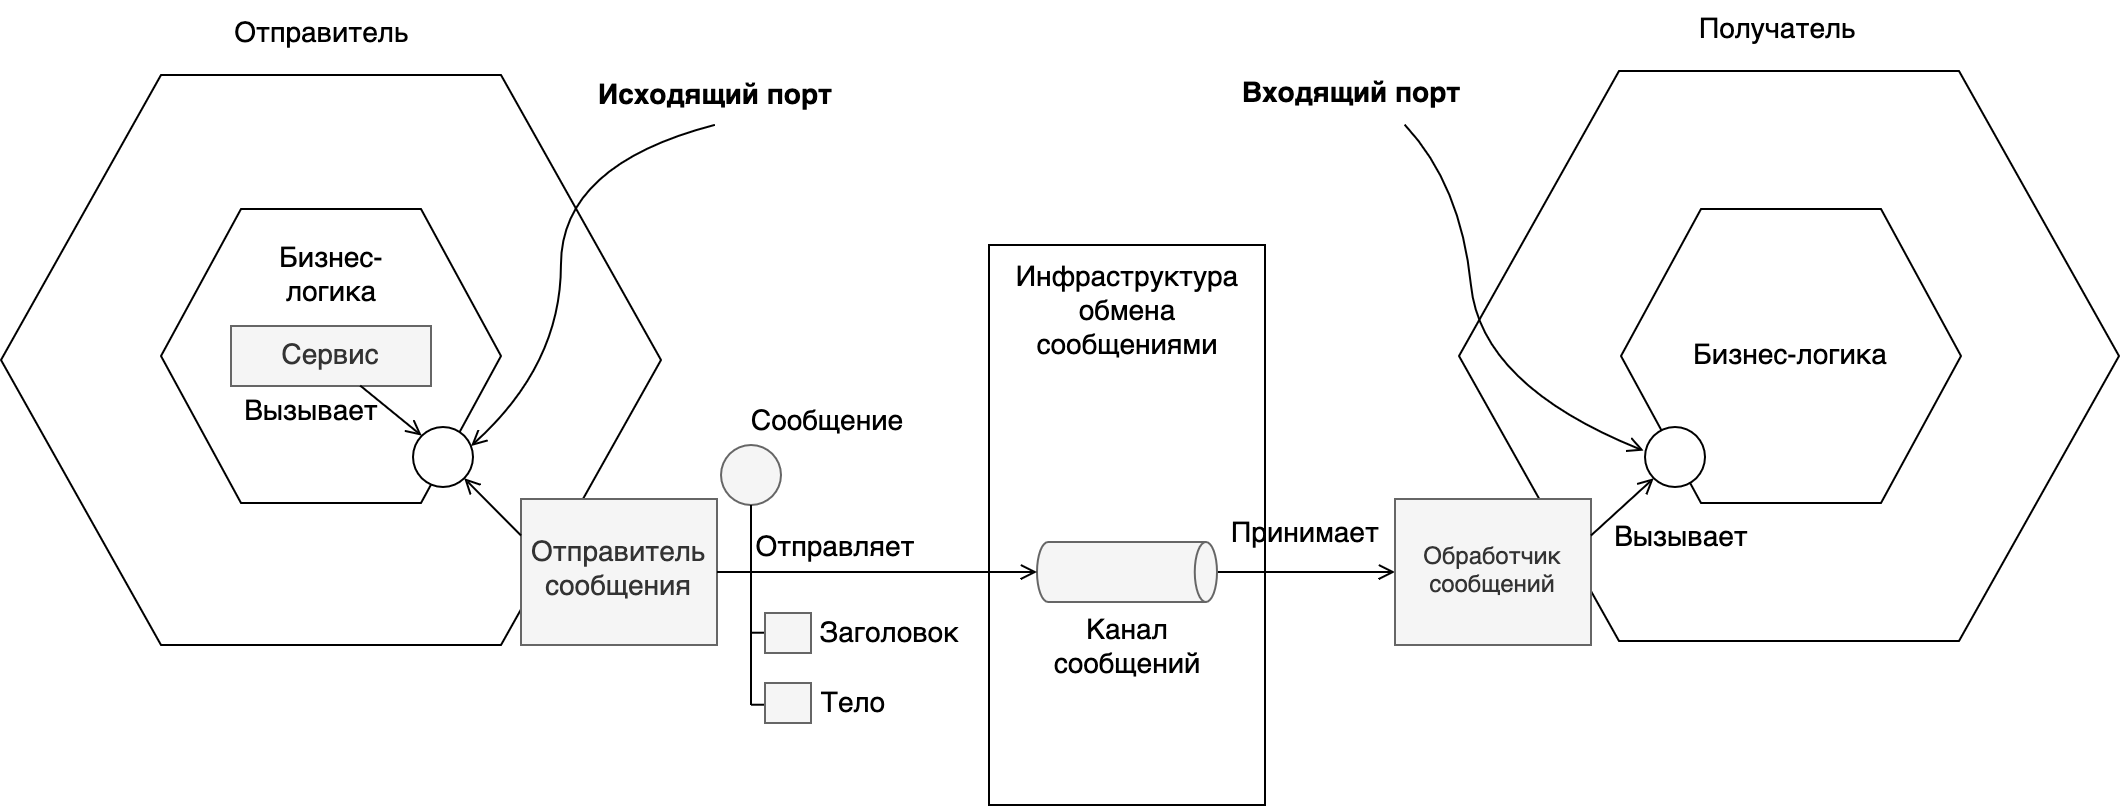
\includegraphics[width=1\linewidth]{assets/microservices-broker-messaging.png}
    \caption{Структура процесса передачи сообщений, используя брокер сообщений}
    \label{fig:microservices-broker-messaging}
\end{figure}

Архитектурный стиль \textit{REST} (\textit{Representational State Transfer}) \textit{API}~-- это стиль для разработки веб-сервисов, который основывается на принципах и ограничениях, способствующих созданию распределённых систем. В контексте веб-программирования, \textit{REST API} представляет собой набор интерфейсов, через которые клиентские приложения могут взаимодействовать с сервером с помощью стандартных \textit{HTTP}-методов, таких как \textit{GET}, \textit{POST}, \textit{PUT}, \textit{DELETE}. Эти методы используются для получения, отправки, обновления или удаления данных. \textit{RESTful}-сервисы обеспечивают лёгкость интеграции и взаимодействия между компонентами системы, поскольку они используют стандартные протоколы передачи данных (например, \textit{JSON} или \textit{XML}).

В \textit{REST} определяется строгое разделение ответственности между компонентами клиент-серверной системы, облегчающее реализацию необходимых актеров (\textit{actors}). Другой целью \textit{REST} является упрощение семантики взаимодействия компонентов сетевых систем, что позволяет улучшить масштабируемость и повысить производительность. В основу \textit{REST} заложен принцип автономности запросов, означающий, что запросы, обрабатываемые клиентом или сервером, должны включать всю контекстную информацию, необходимую для их понимания. При работе \textit{REST}-систем для обмена данными стандартных медиа-типов используется минимальное количество запросов. \textit{REST}-системы используют \textit{URI} (универсальные идентификаторы ресурсов) для поиска и получения доступа к представлениям необходимых ресурсов.

Клиент должен сообщить сервису, куда тому следует вернуть результат, и сопоставить ответное сообщение со своим запросом. Для этого клиент отправляет командное сообщение с каналом ответа в заголовке. Сервер записывает в этот канал свой ответ, содержащий идентификатор соответствия с тем же значением, что и идентификатор запроса. Клиент использует идентификатор соответствия, чтобы сопоставить свое сообщение с ответом.

Как результат, микросервисная архитектура стала неотъемлемой частью любой компании, зависящей от программных технологий.
